\documentclass[class=article,border=5pt,tikz]{standalone}

\begin{document}
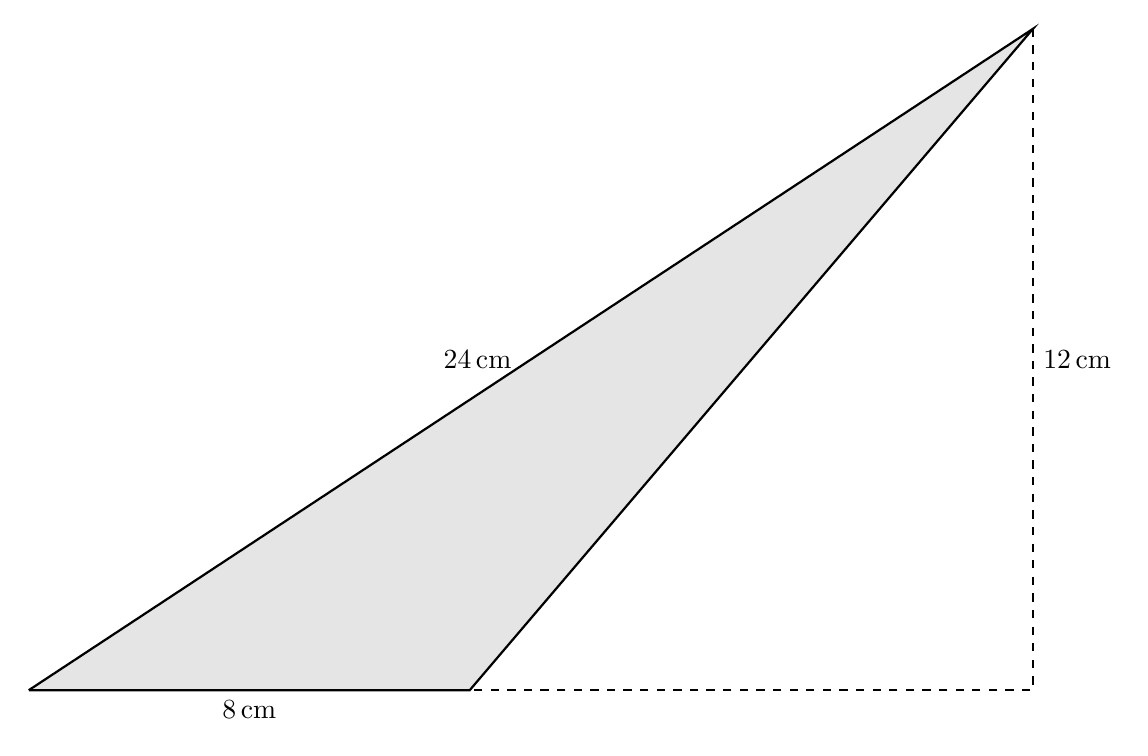
\begin{tikzpicture}[thick,scale=0.7]
\draw [fill=gray!20](0,0) -- (18.22,12) node[midway,left]{$24$\,cm\,\,} -- (8,0)  -- (0,0) node[midway,below]{$8$\,cm};

\draw [dashed] (18.22,12) -- (18.22,0)  node[midway,right]{$12$\,cm} -- (8, 0);
\end{tikzpicture}

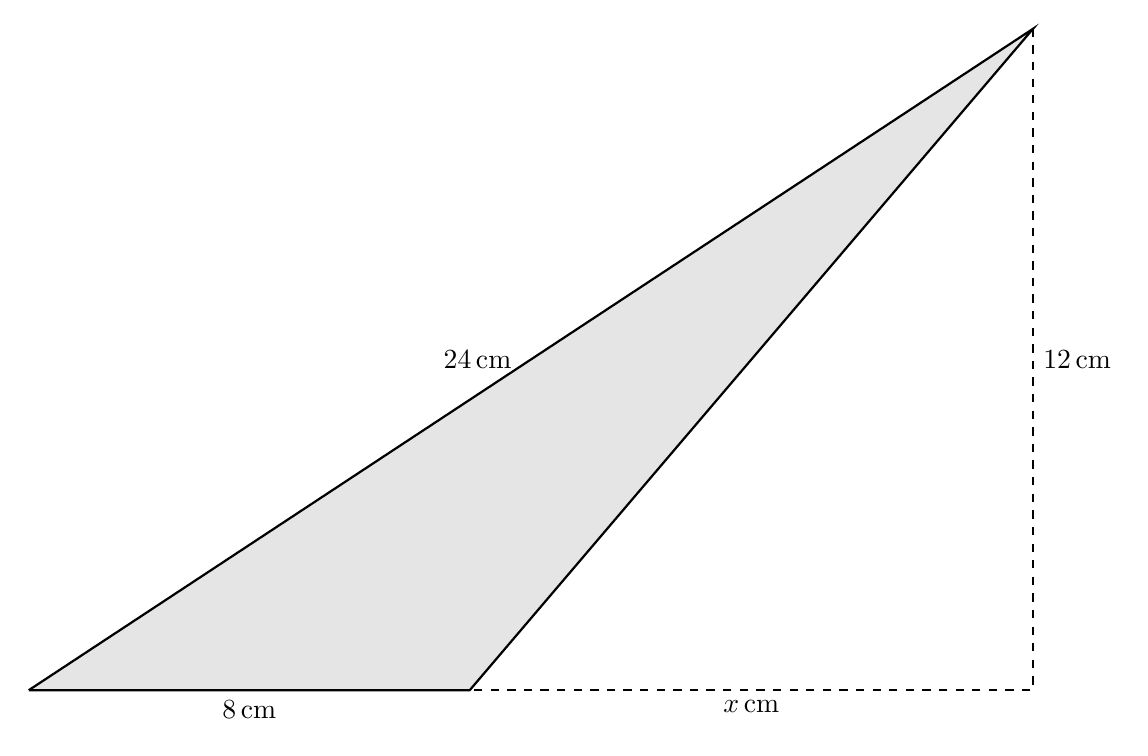
\begin{tikzpicture}[thick,scale=0.7]
\draw [fill=gray!20](0,0) -- (18.22,12) node[midway,left]{$24$\,cm\,\,} -- (8,0)  -- (0,0) node[midway,below]{$8$\,cm};

\draw [dashed] (18.22,12) -- (18.22,0)  node[midway,right]{$12$\,cm} -- (8, 0) node[midway,below]{$x$\,cm};
\end{tikzpicture}
\end{document}

